% concatenated from 260903_ABR_Conjugating_full_cycles_revised.tex
%\documentclass{article}
\documentclass[11pt]{amsart}
\usepackage{graphicx} % Required for inserting images

%\documentclass[11pt]{amsart}
\usepackage[utf8]{inputenc}
\usepackage[margin=1in,letterpaper,portrait]{geometry}
\usepackage{ytableau}
\ytableausetup{notabloids}
\ytableausetup{centertableaux}
\usepackage{latexsym,amsmath,amssymb,verbatim, tikz}
\usepackage{graphicx}
%\usepackage{amsmath, amssymb, tikz}
\usepackage{hyperref}

%\theoremstyle{plain}
   \newtheorem{thm}{Theorem}[section]
   \newtheorem{theorem}{Theorem}[section]
   \newtheorem{proposition}[theorem]{Proposition}
   \newtheorem{prop}[theorem]{Proposition}
   \newtheorem{lemma}[theorem]{Lemma}
   \newtheorem{corollary}[theorem]{Corollary}
   \newtheorem{conjecture}[theorem]{Conjecture}
   \newtheorem{problem}[theorem]{Problem}
   \newtheorem{observation}[theorem]{Observation}
   \newtheorem{obs}[theorem]{Observation}
%\theoremstyle{definition}
   \newtheorem{definition}[theorem]{Definition}
   \newtheorem{defn}[theorem]{Definition}
   \newtheorem{example}[theorem]{Example}
   \newtheorem{examples}[theorem]{Examples}
   \newtheorem{question}[theorem]{Question}
   \newtheorem{remark}[theorem]{Remark}
   

\numberwithin{equation}{section}

\newcommand{\todo}[1]{\vspace{5 mm}\par \noindent
\marginpar{\textsc{ToDo}} \framebox{\begin{minipage}[c]{0.95
\textwidth}
 #1 \end{minipage}}\vspace{5 mm}\par}

\newcommand\comp[2]{\alpha{(#2,#1)}}
\newcommand\ccomp[2]{\alpha^\cyc{(#2,#1)}}

\newcommand{\Q}{{\mathcal {Q}}}

\newcommand{\FF}{{\mathbb {F}}}
\newcommand{\CC}{{\mathbb {C}}}
\newcommand{\QQ}{{\mathbb {Q}}}
\newcommand{\RR}{{\mathbb {R}}}
\newcommand{\ZZ}{{\mathbb {Z}}}
\newcommand{\NN}{{\mathbb {N}}}

\newcommand{\spn}{{\operatorname{span}}}
\newcommand{\Cyl}{\operatorname{Cyl}}
\newcommand{\Tor}{\operatorname{Tor}}

\newcommand{\then}{\Rightarrow}
\newcommand{\ve}{\varepsilon}

\newcommand{\rank}{{\operatorname{rank}}}

\newcommand{\Aut}{{\operatorname{Aut}}}
\newcommand{\Des}{{\operatorname{Des}}}
\newcommand{\cDes}{{\operatorname{cDes}}}
\newcommand{\cyc}{{\operatorname{cyc}}}
\newcommand{\cdes}{{\operatorname{cdes}}}
\newcommand{\des}{{\operatorname{des}}}
\newcommand{\ch}{{\operatorname{ch}}}
\newcommand{\shape}{{\operatorname{shape}}}
\newcommand{\SYT}{{\operatorname{SYT}}}
\newcommand{\co}{{\operatorname{co_n}}}
\newcommand{\cc}{{\operatorname{cc}_n}}

\newcommand{\Inv}{{\operatorname{Inv}}}

\newcommand{\inv}{{\operatorname{inv}}}
\newcommand{\minv}{{\operatorname{minv}}}
\newcommand{\winv}{{\operatorname{winv}}}
\newcommand{\cwinv}{{\operatorname{cwinv}}}
\newcommand{\Einv}{{\operatorname{Einv}}}

\newcommand{\dist}{{\operatorname{dist}}}

\newcommand{\sign}{{\operatorname{sign}}}

\newcommand{\D}{{\operatorname{Diameter}}}
\newcommand{\Sort}{{\operatorname{Sort}}}

\newcommand{\one}{{\mathbf{1}}}

\newcommand{\cs}{{\tilde{s}}}

\newcommand{\xx}{{\mathbf{x}}}
\newcommand{\ttt}{{\mathbf{t}}}
\newcommand{\symm}{{\mathfrak{S}}}

\newcommand{\DDD}{{\mathcal{D}}}
\newcommand{\EEE}{{\mathcal{E}}}
\newcommand{\UUU}{{\mathcal{U}}}
\newcommand{\A}{{\mathcal{A}}}

\newcommand{\F}{\mathcal{F}}

\newcommand{\uX}{\underline{X}}
\newcommand{\uY}{\underline{Y}}
\newcommand{\uYr}{\underline{Y_r}}
\newcommand{\uYi}{\underline{Y_i}}

\newcommand{\edgeright}{{\operatorname{minimal}}}

\newcommand{\AffDes}{{\operatorname{cDes}}}
%\newcommand{\AffDes}{{operatorname{AffDes}}}
%\newcommand{\AffDes}{\widetilde{{operatorname{Des}}}}}

\newcommand{\udots}{\reflectbox{$\ddots$}}

\newlength{\mysizetiny}
\setlength{\mysizetiny}{0.3em}
\newlength{\mysizesmall}
\setlength{\mysizesmall}{0.8em}
\newlength{\mysize}
\setlength{\mysize}{1.3em}%{10pt}%{1.5em}
\newlength{\mysizelarge}
\setlength{\mysizelarge}{2em}

\title[Conjugating full cycles]
{Conjugating full cycles by adjacent transpositions: \\
diameter and sorting time}
%A graph of full cycles}
%\author{Ron M. Adin, Eli Bagno and Yuval Roichman - draft}

\author{Ron M.\ Adin}
\address{Department of Mathematics, Bar-Ilan University, Ramat-Gan 52900, Israel}
\email{radin@math.biu.ac.il}

\author{Eli Bagno}
\address{Jerusalem College of Technology and Michlala College, Jerusalem, Israel}
\email{bagnoe@jct.ac.il}

\author{Yuval Roichman}
\address{Department of Mathematics, Bar-Ilan University, Ramat-Gan 52900, Israel}
\email{yuvalr@math.biu.ac.il}

\date{September 3, 2026}

\subjclass{05A05, 68P10}
\keywords{Sorting, adjacent transpositions, cyclic permutation}

\begin{document}

\begin{abstract}
    We establish upper and lower bounds on the maximal number of steps needed to transform a cyclic permutation to the canonical cyclic permutation  
    using conjugation by adjacent transpositions, and on the diameter of the underlying Schreier graph.  
\end{abstract}

\maketitle

\tableofcontents 

%\maketitle

\section{Introduction}\label{sec:introduction}

%\subsection{The problems}

Let $C_n$ be the set of $n$-cycles in the symmetric group $S_n$. 
Let $\Phi_n := \{s_i = (i,i+1) :\, 1 \le i < n\}$ be the set of adjacent transpositions (Coxeter simple reflections) in $S_n$.

\begin{definition}\label{def:1}
    Consider the undirected graph $\Gamma_n$, with vertex set $C_n$, in which two cycles $c_1,c_2 \in C_n$ are adjacent if $c_2 = s_i c_1 s_i$ for some adjacent transposition $s_i \in \Phi_n$.     
\end{definition}

%\todo{Eli: IMHO, place the definition of diameter before the wording of the problem}

\begin{problem}\label{pb:1}
    Find the diameter of the graph $\Gamma_n$,
    \[
        D_n := \D(\Gamma_n)
        = \max_{\beta,\gamma\in C_n} \dist_{\Gamma_n}(\beta,\gamma).
    \]
Here $ \dist_{\Gamma_n}(\beta,\gamma)$ is the 
distance (length of shortest path) in $\Gamma_n$ between $\beta$ and $\gamma$. 
\end{problem}



%In this note we study the diameter of $\Gamma_n$, denoted by $D_n$.

%\medskip

A closely related problem is the following. 
A {\em cyclic permutation} $[\pi]$ of size $n$ is 
%a presentation of an $n$-cycle $\pi\in S_n$ as  
%on the letters $[n]:=\{1,\dots,n\}$ is a 
%Let $[\pi]$ be a cyclic permutation in $S_n$, represented by
a bijective labeling of $n$ distinct points on a circle 
%of length $n$ 
by the elements of $[n] := \{1, 2,\dots, n\}$; two labelings are equivalent if one can be obtained from the other by a cyclic shift. 
 The {\em canonical cyclic permutation} $c_n: = (1, 2, \dots , n)$ is the one in which the elements are clockwise labeled by $1,\dots,n$. 
%$[n] = \{1, 2,\dots, n\}$. 
A {\it permissible step} on $[\pi]$ is a switching of two consecutive values, $i$ and $i+1$, for some $1 \le i < n$. 

%\todo{Eli: I think that the permutation $\pi$ does not need the brackets unless we want to stress that it is an equivalence class. In this case the definition has to appear in the introduction}.

\begin{definition}\label{df:2}
     The {\em  Coxeter cyclic sorting time}, $\Sort_n$,  is the  maximal number of permissible steps needed to convert a cyclic permutation $[\pi]$ of size $n$ into the canonical cyclic permutation $c_n = (1, 2, \dots , n)$.  
\end{definition}

     By Remark~\ref{rem:iso} below, 
    \[
        \Sort_n
        := \max_{\gamma\in C_n} \dist_{\Gamma_n}(c_n, \gamma). 
    \]   

\begin{problem}\label{pb:2}

%\begin{enumerate}
    % \item 
    % How many permissible steps are 
    % %What is the maximal number of permissible steps 
    % needed in order to convert a cyclic permutation $[\pi]$ into the canonical cyclic permutation $c_n: = (1, 2, \dots , n)$?

%\todo{Eli: IMHO, the cycle $(1,\dots,n)$ should not be called the identity cycle. Maybe the canonical cycle}. 

%    \item 
    Find the  Coxeter cyclic sorting time. 
%\end{enumerate}

\end{problem}

%\todo{
For other sorting processes on cyclic permutations see~\cite{AAR} and references therein. 
%}

%\smallskip

By definition, the  Coxeter cyclic sorting time is not bigger than the diameter.
Since the graph $\Gamma_n$ is not vertex transitive for $n\ge 4$ (see, e.g., Figure~\ref{fig:gamma4}), these two numbers are not necessarily equal. 
For example, for $n=5$, $\D(\Gamma_5)=5>4=\Sort_5$. 

\begin{figure*}[ht]
\begin{center} 
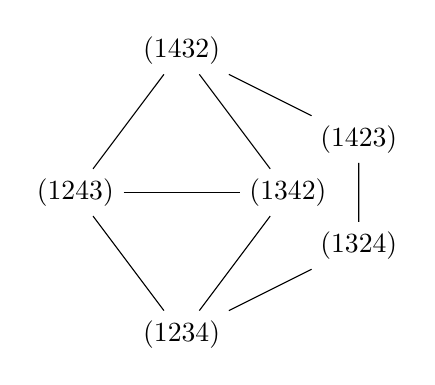
\begin{tikzpicture}[scale=.45]
\node (2) at (0,4) {$(1432)$};
\node (1) at (-3,0) {$(1243)$};
\node (1') at (3,0) {$(1342)$};
\node (0) at (0,-4) {$(1234)$};
\node (A1) at (5,-1.5) {$(1324)$};
\node (A2) at (5,1.5) {$(1423)$};
\draw (2)--(1)--(0)--(1')--(2)--(A2)--(A1)--(0);
\draw  (1)--(1');
\end{tikzpicture}
\end{center}
    \caption{The graph $\Gamma_4$.}
    \label{fig:gamma4}
\end{figure*}

%\todo{Eli: In Fig.1, I don't see what is the meaning of the horizontal line connecting $(1243)$ and $(1342)$.}

In this paper we prove
\begin{theorem}\label{thm:main1}
    For every positive integer $n$, 
    \[
        %%% \frac{(2n-1)(n-1)}{6} 
        %%% \ge \Sort_n  
        %%% \ge (\frac{1}{2} - \frac{\pi}{16}) n^2-n
     %   \frac{(8 - \pi)n^2 - 24n}{16}
         \frac{8-\pi}{16}\cdot n^2 - \frac{3n}{2} %+O(n)
        \le \Sort_n  
        \le \frac{1}{3}\cdot n^2 - \frac{3n-1}{6} %+O(n)
    %    \frac{2n^2-3n+1}{6} 
    \]
    and
    \[
        %%% \frac{3}{8}n^2 - \frac{n}{2} 
        %%% \ge \D(\Gamma_n)
        %%% \ge  (\frac{1}{2} - \frac{\pi}{16}) n^2-n. 
        %\frac{(8 - \pi)n^2 - 24n}{16}
         \frac{8-\pi}{16}\cdot n^2 - \frac{3n}{2} %+O(n)
        \le \D(\Gamma_n)
         \le \frac{3}{8}\cdot n^2 - \frac{4n-1}{8}. %+O(n).
        %\le \frac{3n^2 - 4n+1}{8}.
    \]     
%\begin{enumerate}
%\item
    % \[
    %     % \frac{(2n-1)(n-1)}{6} 
    %     % \ge \Sort_n  
    %     % \ge (\frac{1}{2} - \frac{\pi}{16}) n^2-n
    %     \frac{(8 - \pi)n^2 - 24n}{16}
    %     \le \Sort_n  
    %     \le \frac{2n^2-3n+1}{6} 
    % \]
    % and
    % \[
    %     % \frac{3}{8}n^2 - \frac{n}{2} 
    %     % \ge \D(\Gamma_n)
    %     % \ge  (\frac{1}{2} - \frac{\pi}{16}) n^2-n. 
    %     \frac{(8 - \pi)n^2 - 24n}{16}
    %     \le \D(\Gamma_n)
    %     \le \frac{3n^2 - 4n+1}{8}.
    % \]   
%\item  
%\end{enumerate}
% \todo{YR: To address referee comment, maybe better to state
% %    For every positive integer $n$, 
%     \[
%          \frac{(2n-1)(n-1)}{6} 
%          \ge \Sort_n  
%          \ge (\frac{1}{2} - \frac{\pi}{16}) n^2-n
%      %   \frac{(8 - \pi)n^2 - 24n}{16}
%         %  \frac{8-\pi}{16}\cdot n^2 +O(n)
%         % \le \Sort_n  
%         % \le \frac{1}{3}\cdot n^2 +O(n)
%     %    \frac{2n^2-3n+1}{6} 
%     \]
%     and
%     \[
%          \frac{3}{8}n^2 - \frac{n}{2} 
%          \ge \D(\Gamma_n)
%          \ge  (\frac{1}{2} - \frac{\pi}{16}) n^2-n. 
%         %\frac{(8 - \pi)n^2 - 24n}{16}
%         %  \frac{8-\pi}{16}\cdot n^2 +O(n)
%         % \le \D(\Gamma_n)
%         %  \le \frac{3}{8}\cdot n^2 +O(n).
%         %\le \frac{3n^2 - 4n+1}{8}.
%     \]   
%     }
\end{theorem}




See Theorems~\ref{thm:u0}, ~\ref{thm:2} and~\ref{thm:1} below.
Note that $\frac{8 - \pi}{16} \sim 0.30365$.

% \begin{remark}
%     \(
%         \frac{8 - \pi}{16} \sim 0.303, 
%         \qquad
%         \frac{1}{3} \sim 0.333,
%         \qquad \text{and }
%         \frac{3}{8} = 0.375.
%     \)    
% \end{remark}

\begin{remark}
Theorem~\ref{thm:main1} implies that the diameter and sorting time discussed in this paper, where permissible steps switch adjacent values, are different from those studied in~\cite{AAR}, where steps switch adjacent positions. 
%In particular, unlike $\Gamma_n$, the underlying graph of switching adjacent positions  is vertex transitive. 
\end{remark}



%\todo{A few words on: %relations to:
% (i) other cyclic sorting processes;  %maximal rank of the 
%\noindent
%(ii) {\em  weak orders} on conjugacy classes.   
%of full cycles}
%}




%The graph $\Gamma_n$ can also be seen as the Hasse diagram of a partially ordered set (poset) in the following way: For each $\pi,\sigma \in \Gamma_n$ we say that $\pi \leq \sigma$ if there is a shortest path (a geodetic path) between the cannonical element of $\Gamma_n$, and $\sigma$ which passes through $\pi$.
%Changing the choice of the conjugacy class from the class of full cycles to the class of involutions with or without fixed points, one can find some remarkable results in the literature which give some motivation for this work. 
%As an example, a similar but slightly different poset was studied by Deodar and Srinvasan in \cite{DS}. 
%They considered the Bruhat order on conjugacy classes of involutions and defined the statistic ${\rm wt(\cdot)}$ that serves as a rank function for their poset. 
%Actually, it can be showed, based on \cite{CCT}, that Deodar and Srinvasan's $wt(\pi)$ coincides with the analogue to involutions of the maximal rank we are dealing with here.  










%\medskip

%Consider the following graph: 
%The vertex set is the conjugacy class of long cycles in $S_n$, with an edge connecting $g$ to $s_igs_i$ for each simple reflection (i.e.,  adjacent transposition) $s_i=(i,i+1)$ $(1\le i<n)$.

%\begin{question}\label{q1}
%    Which element is at maximal distance from the cycle $c_n:= (1,2,\dots, n)$ ?
%\end{question}

%%\begin{observation} 

%Here is an equivalent formulation: Let $\sim$ be the equivalence relation on $S_n$ defined by: $\pi \sim \pi c_n^k$ $(\forall k)$, where $c_n:= (1,2,\dots,n)$ as above. For a permutation $\pi\in S_n$, the {\em cyclic permutation} $[\pi]$ is the equivalence class of $\pi$ in $S_n$; equivalently, a conjugacy class of $\ZZ_n = \langle c_o \rangle$ in $S_n$.  Question~\ref{q1} is equivalent to the following.

%\begin{question}\label{q2}
%    Which $[\pi]$ has largest
%    \[
%        \minv([\pi]) 
%        := \min \{\inv(\pi c_n^k) :\, k \in \ZZ\} ?
%    \]
%\end{question}

%%\end{observation}




\section{Notation and preliminaries}

Let $S_n$ be the symmetric group on the letters $[n]:=\{1,\dots, n\}$. The one-line notation of a permutation $\pi\in S_n$ is denoted by square brackets $[\pi(1),\dots,\pi(n)]$, while the cycle notation by parentheses. For example $[3,5,6,1,2,4]=(1,3,6,4)(2,5)\in S_6$.

Letting $H$ be a subgroup of a finite group $G$, and $S\subseteq  G$, the {\em Schreier graph} $X(G/H,S)$ is the undirected graph whose vertex set consists of all left cosets $G/H:=\{\pi H\, :\, \pi\in G\}$; the edges are the unordered pairs $(\pi H, s\pi H)$, for $s\in S, \pi\in G$. 



\section{The minv statistic}

%\subsection{The Schreier graph $X(S_n/\ZZ_n, \Phi_n)$}\label{sec:Schreier}

Let $c_n:=(1,2,\dots,n)=s_1s_2\cdots s_{n-1}\in S_n$. 
Denote by $\ZZ_n$ the cyclic subgroup of $S_n$ generated by $c_n$. Recall the graph $\Gamma_n$ from Definition~\ref{def:1}.

%\begin{observation}
%%\begin{itemize}
%%\item[1.]    
%The graph $\Gamma_n$ is isomorphic to the Schreier graph $X(S_n/\ZZ_n, \Phi_n)$, where $\Phi_n$ is the set of simple reflections in $S_n$. 
%%\item[2.] 
%%\end{itemize}
%\end{observation}

%\begin{remark}\label{rem:iso}
 %   Consider the map from $C_n$ to the set of left cosets $S_n/\ZZ_n$, defined as follows: a cycle $\gamma = (a_1,\dots,a_n)\in C_n$ is mapped  to the coset $\bar\gamma \ZZ_n$, where $\bar\gamma$ is the permutation in $S_n$ defined  by $\bar\gamma(i) = a_i$ $(\forall i)$. This map is a well defined bijection, and induces an isomorphism from the graph $\Gamma_n$ to the Schreier graph $X(S_n/\ZZ_n, \Phi_n)$, where edge multiplicity is ignored. 
%\end{remark}

\begin{remark}\label{rem:iso}
    Consider the map from $C_n$ to the set of left cosets $S_n/\ZZ_n$, defined as follows: a cycle $\gamma = (a_1,\dots,a_n)\in C_n$ is mapped to the coset $\bar\gamma \ZZ_n$, where $\bar\gamma=[a_1,\dots,a_n]$ . This map is a well-defined bijection and induces an isomorphism from the graph $\Gamma_n$ to the Schreier graph $X(S_n/\ZZ_n, \Phi_n)$, where edge multiplicity is ignored. 
\end{remark}




%\subsection{%The minv and einv statistics Cyclic inversion numbers}\label{sec:minv}

Recall the {\em inversion number} of a permutation $\pi\in S_n$,
\[
    \inv(\pi) := |\{i<j :\, \pi(i) > \pi(j)\}|.
\]

\begin{definition}\label{def:2}
    Define the {\em minv} statistic on the left cosets of $\ZZ_n$ in $S_n$ as follows:
    \[
        \minv(\pi \ZZ_n) := \min\{ \inv(\sigma) :\, \sigma \in \pi\ZZ_n)\}
        \qquad (\forall\, \pi\ZZ_n \in S_n/\ZZ_n).
    \]
\end{definition}



%Recall the full cycle $c_n:=(1,2,\dots,n)$.

%The following lemma extends Corollary~\ref{lem:1}.

\begin{lemma}\label{lem:2} 
    For every pair of full cycles $\gamma_1, \gamma_2\in C_n$,
    \[
        \dist_{\Gamma_n}(\gamma_1,\gamma_2)=\min 
        \{\inv(\sigma):\ \sigma \in \bar\gamma_1 \ZZ_n \bar\gamma_2^{-1}\},  
    \]
%\[
%\dist_{\Gamma_n}(\gamma_1,\gamma_2)=\min 
%\{\inv(\bar\gamma_1 c_n^i \bar\gamma_2^{-1}):\ 0\le i<n \},  
%\]
    where $\bar\gamma_1, \bar\gamma_2$ are defined as in Remark~\ref{rem:iso}. 
%the permutation obtained from $\gamma_i$ by erasing the brackets. 
\end{lemma}

\begin{proof} 
    By Remark~\ref{rem:iso}, the distance $\dist_{\Gamma_n}(\gamma_1, \gamma_2)$  
    is equal to the smallest nonnegative integer $\ell$ for which there exist simple reflections $s_{i_1},\ldots,s_{i_\ell}$ satisfying  $s_{i_\ell} \cdots s_{i_1} \bar\gamma_1\ZZ_n = \bar\gamma_2\ZZ_n$.  
    Equivalently, 
    \[
        \ell 
        = \min \{\inv(\tau_2 \tau_1^{-1}) :\, \tau_1 \in \bar\gamma_1\ZZ_n,\, \tau_2 \in \bar\gamma_2\ZZ_n\}
        = \min \{\inv(\sigma) :\, \sigma \in \bar\gamma_2 \ZZ_n \bar\gamma_1^{-1}\}.
        \qedhere
    \]
\end{proof}

\begin{corollary}\label{lem:1} 
    For every full cycle $\gamma \in C_n$
    \[
        \dist_{\Gamma_n}(c_n, \gamma) = \minv(\bar\gamma\ZZ_n),   
    \]
    where $c_n = (1,2,\dots,n) \in C_n$ and $\bar\gamma\ZZ_n \in S_n/\ZZ_n$ is defined as in Remark~\ref{rem:iso}.\\
    In particular, for every $n\ge 1$ 
    \[
        \Sort_n
        = \max_{\pi\in S_n} \minv(\pi \ZZ_n) .
        %: \ \pi\in S_n\}.
    \]
\end{corollary}

We conclude that Problem~\ref{pb:2} is equivalent to the following one. 

\begin{problem}
%\begin{itemize}

%    \item[1.]  
    What is the maximal value of {\em minv} on $S_n/\ZZ_n$ ?
    
%    \item[2.]  
%    What is the expected value of {\em minv} on $S_n/\ZZ_n$ ?

%\end{itemize}
\end{problem}


\section{Upper bound on the Coxeter cyclic sorting time}\label{sec:upper sorting}%\ \\

%Recall definitions and notation from Sections~\ref{sec:introduction} and~\ref{sec:minv}. 
%Denote the diameter of $\Gamma_n$ by $D_n$. 

%Consider the full cycle $c_n:=(1,2,\dots,n)\in S_n$, 
%and denote by $\ZZ_n$ the subgroup generated by $c_n$. 
%Recall the Schreier graph $\Gamma_n:=X(S_n/\ZZ_n,S)$, where $S$ is the Coxeter generating set of the symmetric group $S_n$. 


Recall the  Coxeter cyclic sorting time, $\Sort_n$, from Definition ~\ref{df:2}. The main result in this section is the following. 

% \todo{Eli: No need to recall IMHO. $Sort_n$ was mentioned at the end of the former section}


%In this section we prove the following.

\begin{theorem}\label{thm:u0}
        For every $n\ge 1$,
    \[
        \Sort_n %=\max_{\pi\in S_n}\dist_{\Gamma_n}(\ZZ_n,\pi \ZZ_n)
        % \le \frac{(2n-1)(n-1)}{6}.
        \le \frac{2n^2 - 3n + 1}{6}.
    \]
\end{theorem}

% \todo{Eli: The numerator appeared as $2n^2-3n+1$ in the introduction}

Theorem~\ref{thm:u0} is an immediate consequence of the following result. 

%\begin{definition}\label{def:22}
%For $\pi\in S_n$, let $\Einv([\pi])$ be the expected value of $\inv$ on $\pi \ZZ_n$. Namely, 
%\[
%\Einv(\pi \ZZ_n):=E_{ \sigma \in  \pi \ZZ_n}\{ \inv(\sigma)\}.
%\]
%\end{definition}

%\begin{definition}\label{def:22}
%    For $\pi\in S_n$, let $\Einv([\pi])$ be the expected value of $\inv$ on $\pi \ZZ_n$. Namely, 
%    \[
%        \Einv(\pi \ZZ_n):=E_{ \sigma \in  \pi \ZZ_n}\{ \inv(\sigma)\}.
%    \]
%\end{definition}


%For a permutation $\pi\in S_n$ denote the expected value of $\inv$ on $\pi \ZZ_n$ by $\Einv(\pi)$, see Definition~\ref{def:22}. 

\begin{proposition}\label{prop:u0}
    For every $n\ge 1$, the maximum of the expected value of $\inv$ on left cosets $\pi \ZZ_n$ satisfies 
    \[
        \max_{\pi \in S_n} E\{ \inv(\sigma): \sigma \in  \pi \ZZ_n\}
        %\Einv([\pi])
        = \frac{(2n-1)(n-1)}{6}.
    \]
\end{proposition}

See Remark~\ref{rem:max} below.

\begin{proof}[Proof of Theorem~\ref{thm:u0}]
    By %Remark~\ref{rem:iso}, 
    Corollary~\ref{lem:1}, Definition~\ref{def:2} 
    and Proposition~\ref{prop:u0},
    %, and Lemma~\ref{lem:u7} together with Corollary~\ref{obs:u5} 
\begin{align*}
    \Sort_n 
    % &= \max_{\gamma\in C_n} \dist_{\Gamma_n}(c_n,\gamma)
    &= \max_{\pi\in S_n} \minv(\pi \ZZ_n)
    = \max_{\pi\in S_n} \min \{\inv(\pi c_n^i): 0\le i<n\} \\
    &\le \max_{\pi\in S_n} E\{\inv(\pi c_n^i): 0\le i<n\}
    %= \max_{\pi \in S_n} \Einv([\pi])
    = \frac{(2n-1)(n-1)}{6}. 
    \qedhere
\end{align*}
%\[
%=
%\frac{1}{n}\left(\max_{\pi\in S_n} \cwinv(\pi)
%+\binom{n+1}{3}\right)
%=
%\frac{1}{n}\left(\binom{n}{3}+\binom{n+1}{3}\right)= \frac{(2n-1)(n-1)}{6}.
%\]

\end{proof}


In order to prove Proposition~\ref{prop:u0} 
%Theorem~\ref{thm:u0} 
we consider a weighted version of the inversion number, as well as a cyclic variant, see Definitions~\ref{def:winv} and~\ref{def:cyclic winv} below. 
%introduce the {\em cyclic weighted inversion number}.

\begin{defn}\label{def:winv}
    The {\em weighted inversion number} of a permutation $\pi\in S_n$ is 
    \[
        \winv(\pi)
        := \sum_{\substack{i,j \\ i<j,\, \pi(i)>\pi(j)}} (\pi(i)-\pi(j)).
    \]
\end{defn}

\begin{lemma}\label{lem:u6}
    For every $\pi \in S_n$,
    \[
        % \sum_{i=1}^n i\cdot \pi(i) = \sum_{i=1}^n i^2-\winv(\pi) 
        % = \frac{n(n+1)(2n+1)}{6}-\winv(\pi).
        \winv(\pi) 
        = \sum_{i=1}^n i^2 -
        \sum_{i=1}^n i\cdot \pi(i) .
    \]
\end{lemma}

\begin{proof}
    By induction on the inversion number $\inv(\pi)$. 
    If $\inv(\pi) = 0$ then $\pi = id$, and the claim clearly holds. 
    Now assume that the claim holds for all $\pi' \in S_n$ with $\inv(\pi') \le k$, and let $\pi \in S_n$ have $\inv(\pi) = k+1$. 
    Since $\pi \ne id$, there exists $1 \le j<n$ such that $\pi(j) > \pi(j+1)$, so that $\pi' := \pi s_j$ satisfies
    $\inv(\pi') = k$. 
    % Switching $i$-th and $i+1$-st letters in $\pi s_i$ changes both handsides by $\pi(i)-\pi(i+1)$. Proof is completed.
    By the induction hypothesis,
    \[
        \winv(\pi') 
        = \sum_{i=1}^n i^2 -
        \sum_{i=1}^n i\cdot \pi'(i) .
    \]    
    By Definition~\ref{def:winv}, $\winv(\pi) - \winv(\pi') = \pi(j) - \pi(j+1)$. Also,
    \[
        \left( \sum_{i=1}^n i^2 -
        \sum_{i=1}^n i\cdot \pi(i) \right)
        - \left( \sum_{i=1}^n i^2 -
        \sum_{i=1}^n i\cdot \pi'(i) \right)
        = \sum_{i=1}^n i \cdot \left( \pi'(i) - \pi(i) \right)
        = \pi(j) - \pi(j+1),
    \]
    and thus the claim holds for $\pi$ as well.
    This completes the induction step and the proof.
\end{proof}

Denote $w_0:=[n,n-1,\dots,1]\in S_n$. Recall that $w_0$ has the largest inversion number in $S_n$. 
% By Definition~\ref{def:winv},  

\begin{observation}\label{obs:u2}
    For any $\pi \in S_n$,
    % \begin{enumerate}
    %     \item   
        % For every $\pi\in S_n$,
        \[
            \winv(\pi)+\winv(\pi w_0)
            = \sum_{1 \le k < \ell \le n} (\ell - k)
            % = \sum_{\ell = 2}^{n} \sum_{k=1}^{\ell-1} (\ell - k)
            = \sum_{\ell = 2}^{n} \binom{\ell}{2} = \binom{n+1}{3}
        \]
        and
        % \item    
        % For every $\pi\in S_n\setminus\{id,w_0\}$,
        \[
            0 = \winv(id) 
            \le \winv(\pi)
            \le \winv(w_0)
            = \binom{n+1}{3}.
        \]
    % \end{enumerate}
\end{observation}

%\begin{proof}
%The left inequality is proved by induction on $\inv(\pi)$, noting that if 
%$\inv(\pi)<\inv(\pi s_i)$, for some Coxeter generator $s_i:=(i,i+1)$, $1\le i<n$, then $\winv(\pi)<\winv(\pi s_i)$. 
%The left inequality implies the right inequality. 
%is proved by induction on $\inv(w_0 \pi^{-1})=\inv(w_0)-\inv(\pi)$. 
%\end{proof}
%\todo{Eli: I don't understand.  The left inequality is trivial since $\winv(id)=0$. }
The following cyclic variant of $\winv$ plays a key role in the proof.

\begin{defn}\label{def:cyclic winv}
    The {\em cyclic weighted inversion number} of a permutation $\pi\in S_n$ is
    \[
        \cwinv(\pi)
        := n\cdot \inv(\pi)-2\cdot \winv(\pi)
        = \sum_{\substack{i,j \\ i<j,\, \pi(i)>\pi(j)}} (n-2\pi(i) + 2\pi(j)).
    \]
\end{defn}

The following observation justifies the adjective {\em cyclic} in Definition~\ref{def:cyclic winv}. 

\begin{observation}\label{obs:u3}
The cyclic weighted inversion number is invariant under cyclic shifts; namely, 
% letting $c_n:=(1,2,\dots,n)$ %then 
\[
    \cwinv(\pi c_n) = \cwinv(\pi) 
    \qquad (\forall \pi\in S_n).
\]
\end{observation}

\begin{proof}
    Denote $m:=\pi(1)$. Then $m = \pi c_n(n)$, so that
    \[
        \inv(\pi c_n)-\inv(\pi)
        = (n-m)-(m-1) = n+1-2m
    \]
    and
    \[
        \winv(\pi c_n)-\winv(\pi)
        = \sum_{m < j \le n} (j-m) -\sum_{1 \le j < m} (m-j)
        = \binom{n-m+1}{2} - \binom{m}{2}.
    \]
    Thus
    \[
        \cwinv(\pi c_n)-\cwinv(\pi)
        = n(n+1-2m)-(n-m+1)(n-m)+m(m-1)
        = 0. \qedhere
    \]
\end{proof}
%\begin{proof}
%Denote $k:=\pi(1)$. Then
%    \[
%    \cwinv(\pi c_n^{-1})-\cwinv(\pi)=(n-k)(n+2k)-2\sum_{j>k}j -(k-1)(n-2k)-2\sum_{j<k}j=0.
%    \]
%\end{proof}

\begin{observation}\label{obs:u4}
    For every $\pi\in S_n$
    \[
    \cwinv(\pi)+\cwinv(\pi w_0)= n\binom{n}{2}-2\binom{n+1}{3}=\binom{n}{3}.
    \]
\end{observation}

\begin{corollary}\label{obs:u5}
    For every $\pi\in S_n$
    \[
    0=\cwinv(id)\le \cwinv(\pi)\le \cwinv(w_0)=
    %n\binom{n}{2}-2\binom{n+1}{3}=
    \binom{n}{3}.
    \]
\end{corollary}

\begin{proof}
    By Observation~\ref{obs:u3}, we may assume that $\pi(n)=n$.
    Let $\bar\pi=[\pi(1),\dots,\pi(n-1)]\in S_{n-1}$. By definition,
    \[
    \cwinv(\pi)=n\cdot \inv(\pi)-2\cdot \winv(\pi)=
    n\cdot \inv(\bar \pi)-2\cdot \winv(\bar \pi)=
    \cwinv(\bar \pi)+ \inv(\bar \pi).
    \]
Hence, 
\[
\max_{\pi\in S_n} \cwinv(\pi)\le \max_{\bar \pi\in S_{n-1}} \cwinv(\bar \pi)+\max_{\pi \in S_{n-1}}\inv(\pi). 
\]
By iteration, 
\[
    \max_{\pi\in S_n} \cwinv(\pi)
    \le \max_{\bar \pi\in S_{n-1}} \cwinv(\bar \pi)+\max_{\pi \in S_{n-1}}\inv(\pi)
    \le \sum_{j=1}^{n-1} \max_{\pi\in S_j} \inv(\pi)
    = \sum_{j=1}^{n-1}\binom{j}{2}
    = \binom{n}{3} 
    = \cwinv(w_0).
\]
Combining this upper bound with Observation~\ref{obs:u4}, 
\[
    \min_{\pi\in S_n} \cwinv(\pi)
    = \binom{n}{3}-\max_{\pi\in S_n}\cwinv(\pi)
    % \ge \binom{n}{3}-\cwinv(w_0) 
    \ge 0 
    = \cwinv(id). \qedhere
\]
\end{proof}


\begin{lemma}\label{lem:u7}
    For every $\pi \in S_n$
    \[
        n\cdot  %\max_{\pi \in S_n} 
        E\{ \inv(\sigma): \sigma \in  \pi \ZZ_n\}
        = \sum_{i=1}^n \inv(\pi c_n^i)
        = \cwinv(\pi)+ \binom{n+1}{3}.
    \]
\end{lemma}

\begin{proof}
% The proof follows from the fact that
% \[
% \inv(\pi c_n^{-1})= \inv(\pi)-n-1+2\pi(n). 
% \]
As in the proof of Observation~\ref{obs:u3},
\[
    \inv(\pi c_n) 
    = \inv(\pi) + n + 1 - 2\pi(1). 
\]
Thus, by iteration
% \[
% \inv(\pi c_n^{-i})= \inv(\pi)-i(n+1)+2\sum\limits_{j=0}^{i-1}\pi(n-j).
% \]
\[
    \inv(\pi c_n^i)
    = \inv(\pi) + \sum_{j=1}^{i} (n + 1 - 2\pi(j)).
\]
Summing over $1\le i\le n$ we obtain
% \begin{align*}
%     \sum\limits_{i=1}^n \inv(\pi c_n^i) 
%     = \sum\limits_{i=1}^n \inv(\pi c_n^{-i})
%     &= \sum\limits_{i=1}^n \left(\inv(\pi)+2\sum\limits_{j=0}^{i-1}\pi(n-j)-i(n+1)\right) \\
%     &= n\cdot \inv(\pi)+2\sum\limits_{i=1}^n \sum\limits_{j=0}^{i-1}\pi(n-j)-(n+1)\binom{n+1}{2} \\
%     &= n\cdot\inv(\pi)+2\sum\limits_{i=1}^n i\cdot \pi(i)-(n+1)\binom{n+1}{2}.
% \end{align*}
\begin{align*}
    \sum_{i=1}^n \inv(\pi c_n^i)
    % &= \sum_{i=1}^n \left( \inv(\pi) + i(n+1) - 2\sum_{j=1}^{i}\pi(j) \right) \\
    &= n \cdot \inv(\pi) + \sum_{i=1}^n \sum_{j=1}^{i} (n + 1 - 2\pi(j)) \\
    &= n \cdot \inv(\pi) + \sum_{j=1}^{n}(n + 1 - j)(n + 1 - 2\pi(j)) \\
    &= n \cdot \inv(\pi) + \sum_{j=1}^{n} j \cdot 2\pi(j) - (n+1) \sum_{j=1}^{n} (2\pi(j) + j) + n(n+1)^2 \\
    &= n \cdot \inv(\pi) + 2\sum_{j=1}^{n} j \cdot \pi(j) - \frac{1}{2}n(n+1)^2
\end{align*}
By Lemma~\ref{lem:u6} and Definition~\ref{def:cyclic winv}, this is equal to
\[
    n \cdot \inv(\pi) + 2\sum_{j=1}^{n} j^2 - 2 \cdot \winv(\pi) - \frac{1}{2}n(n+1)^2
    = \cwinv(\pi)+\binom{n+1}{3}. \qedhere
\]
% Proof is completed.
\end{proof}


\begin{proof}[Proof of Proposition~\ref{prop:u0}]
    By Lemma~\ref{lem:u7} and Corollary~\ref{obs:u5},  
    \begin{align*}
        \max_{\pi \in S_n} E\{ \inv(\sigma): \sigma \in  \pi \ZZ_n\}
    =& \frac{1}{n}\left(\max_{\pi\in S_n} \cwinv(\pi) + \binom{n+1}{3}\right)\\
    =& \frac{1}{n}\left( \binom{n}{3} + \binom{n+1}{3} \right)
    = \frac{(2n-1)(n-1)}{6}.   \qedhere 
\end{align*}
\end{proof}


%\begin{proof}[Proof of Theorem~\ref{thm:u0}]
%    By Corollary~\ref{lem:1}, and Lemma~\ref{lem:u7} together with Corollary~\ref{obs:u5} 
%\[
%\max_{\pi\in S_n}\dist_{\Gamma_n}(\ZZ_n,\pi\ZZ_n)=\max_{\pi\in S_n} \min_{0\le i<n} \{\inv(\pi c_n^i)\}\le \max_{\pi\in S_n}  E\{\inv(\pi c_n^i): 0\le i<n\}
%\]
%\[
%=
%\frac{1}{n}\left(\max_{\pi\in S_n} \cwinv(\pi)
%+\binom{n+1}{3}\right)
%=
%\frac{1}{n}\left(\binom{n}{3}+\binom{n+1}{3}\right)= \frac{(2n-1)(n-1)}{6}.
%\]


%\section{Lower bound}

%\begin{theorem}\label{thm:2}
%    For every $n\ge 1$
%    \[
%    D_n \ge \max_{\gamma\in C_n}\dist_{\Gamma_n}(c_n,\gamma)\ge (\frac{1}{2}-\frac{\pi}{16}) n^2 + O(n).
%    \]
%\end{theorem}


%\begin{proof}[Proof of Theorem~\ref{thm:2}]\ \\
%  \todo{Insert proof}   
%\end{proof}

\begin{remark}\label{rem:max}
    By Corollary~\ref{obs:u5} and Lemma~\ref{lem:u7}, the maximum of the expected value of the inversion number on a $\ZZ_n$-coset is attained at $w_0 \ZZ_n$. However, surprisingly, the maximal value of the statistic $\minv$ 
    (which, by Corollary~\ref{lem:1}, is equal to $\Sort_n$)
    is not attained at this coset, since %\dist_{\Gamma_n}(c_n,w_0)(w_0) = 
    $\minv(w_0 \ZZ_n) = \binom{\lceil n/2\rceil}{2} + \binom{\lfloor n/2\rfloor}{2} = \left\lfloor \frac{(n-1)^2}{4} \right\rfloor $ is strictly less than the lower bound proved in the next section (Theorem~\ref{thm:2}). 
\end{remark}


\section{Lower bound on the Coxeter cyclic sorting time}

In this section we prove the following lower bound on $\Sort_n$, and thus on $\D(\Gamma_n)$ as well.

\begin{theorem}\label{thm:2}
    For every $n\ge 1$
    \[
    %D_n \ge  
    \Sort_n 
    %\max_{\gamma\in C_n}\dist_{\Gamma_n}(c_n,\gamma)
    \ge \left( \frac{1}{2}-\frac{\pi}{16} \right) n^2 -\frac{3}{2} n. % +O(1).
    %+ O(n).
    \]
\end{theorem}

%Since $\D(\Gamma_n) \ge \Sort_n$.

The proof of this theorem uses the following characterization.
% is used in the proof of Theorem~\ref{thm:2}.
%In the proof of Theorem~\ref{thm:2} we will use the following lemma. %which strengthens Lemma~\ref{lem:3} in the case  $\sigma=id$.

\begin{lemma}\label{lem:lower1}
    For every $\pi\in S_n$, $\inv(\pi)=\minv(\pi\ZZ_n)$ if and only if $\pi$ is ``heavy tailed'', namely if, for all $1\le k\le n$, the sum of the last $k$ entries of $\pi$ is at least $\frac{k(n+1)}{2}$;
    % :
    % \[
    %     \sum_{j=1}^{k} \pi(n+1-j) \ge k(n+1)/2
    %     \qquad (\forall k); 
    % \]
    equivalently if, for all $1\le k\le n$, the sum of the first $k$ entries of $\pi$ is at most $\frac{k(n+1)}{2}$:
    \[
        \sum_{j=1}^{k} \pi(j) \le \frac{k(n+1)}{2}
        \qquad (\forall k);
   \]
%For every pair $\pi\in S_n$, there exists $\tau\in \pi \ZZ_n$, such that for every $1\le k\le n$
%\[
%\sum\limits_{i=1}^k \tau(i)\le \frac{k(n+1)}{2}. 
%\]
\end{lemma}

\begin{proof} 
    For every $1\le k\le n$, $\inv(\pi)\le \inv(\pi c_n^k)$ if and only if 
    %    \[
    %    0\le \inv(\pi c_n^k)-\inv(\pi)= \sum\limits_{j=0}^k (n+1-2\pi(j))= k(n+1)-2\sum\limits_{j=1}^k \pi(j). 
    %    \]
    \begin{align*}
        0 \le \inv(\pi c_n^k) - \inv(\pi) 
        =& \sum_{j=1}^{k} \left( \inv(\pi c_n^j) - \inv(\pi c_n^{j-1}) \right) \\
        =& \sum_{j=1}^k \left( (n - \pi c_n^{j-1}(1)) - (\pi c_n^{j-1}(1) - 1) \right) \\
        % = \sum_{j=1}^k \left( n-\pi(j) -(\pi(j)-1) \right) \\
        =& \sum_{j=1}^k (n+1-2\pi(j))
        = k(n+1) - 2\sum_{j=1}^k \pi(j). 
        \qedhere
    \end{align*}
\end{proof}

%\todo{Eli: 
%First: IMHO the sum has to begin in $j=1$.  What is the meaning of $\pi(0)$? 
%Secondly: 
%I suggest adding some self-explaining steps in this equality; something like $$
%$$
%    0\le \inv(\pi c_n^k)-\inv(\pi)=
%    \sum\limits_{j=1}^k(\inv(\pi c_n^j)
%    -\inv(\pi c_n^{j-1}))=$$
%    $$\sum\limits_{j=1}^k (n-(\pi c_n^j)(1)-((\pi c_n^{j-1})(1)-1))=
%    \sum\limits_{j=1}^k (n-\pi(j)-(\pi(j)-1))=$$
%    $$\sum\limits_{j=1}^k (n+1-2\pi(j))=k(n+1)-2\sum\limits_{j=1}^k \pi(j)$$
%\sum\limits_{j=1}^k (n+1-2\pi(j))=}))=\sum\limits_{j=1}^k (n+1-2\pi(j))= k(n+1)-2\sum\limits_{j=1}^k \pi(j)=. 
    %$$}
%}
\begin{proof}[Proof of Theorem~\ref{thm:2}]
    By Corollary~\ref{lem:1}, if $\pi \in S_n$ satisfied the conditions of Lemma~\ref{lem:lower1} then
    \[
        \Sort_n
        \ge \minv(\pi \ZZ_n) 
        = \inv(\pi).
        %: \ \pi\in S_n\}.
    \]
To get a good lower bound, 
%By Corollary~\ref{lem:1}, we need 
we shall construct such a permutation $\pi\in S_n$ with a large  $\inv(\pi)$.
%, which satisfies the conditions of Lemma~\ref{lem:lower1}.    
% to maximize $\inv(\pi)$ over all the permutations $\pi\in S_n$ which satisfy the conditions of Lemma~\ref{lem:lower1}.

% \todo{YR: The definition of $\pi_0$ was unified to hold for $n$ even and odd, to have the statement of Conjecture~\ref{conj:0}  more natural and easier to read.\\
% I have chosen $m:=\lfloor n/2 \rfloor$ and not $m:=\lceil n/2 \rceil$, %although it is less natural for the definition of $\pi_0$, 
% since it is more convenient for computations in the sequal, in particular, the limits of the integral are the same for $n$ odd and even.}

Recall the permutation $w_0 = [n,\ldots,1]$ and consider, as a first approximation, its cyclic shift $w_0 c_n^{m} =[n-m,\ldots,1,n,\ldots,n-m+1]$, where $m:=\lfloor n/2\rfloor$.  
Noting that $w_0 c_n^{m}$ satisfies the conditions of Lemma~\ref{lem:lower1}, one concludes that
\[
    \minv(w_0\ZZ_n)
    = \inv(w_0 c_n^{m})
    = \binom{n-m}{2}+\binom{m}{2}=\binom{\lceil n/2\rceil}{2}+\binom{\lfloor n/2 \rfloor}{2}.
\]
Now, take $w_0 c_n^{m}$ and push the letter $n$ to the left %backwards 
as much as possible, say to position $k_1 + 1$, so that the conditions of Lemma~\ref{lem:lower1} are still satisfied.
Then push the letter $n-1$ to the left as much as possible, say to position $k_2 + 2$, and so on. We obtain the permutation
\begin{align}\label{eq:defpi}
    \pi_0
    &:= \left[
    n-m,n-m-1,\dots, n-m-(k_1-1),n,n-m-k_1,\dots, n-m-(k_2-1),n-1, \right. \\
    & \quad\; \left. n-m-k_2,\dots, 
    n-m-(k_t-1),n+1-t,n-m-k_t,\dots \right] \in S_n, \nonumber
\end{align}
where $0 \le k_1 \le \ldots \le k_{m} \le n-m$ have the minimal possible values such that $\pi_0$ still satisfies the conditions of Lemma~\ref{lem:lower1}. In the sequel we shall obtain explicit expressions for these minimal values, for each $n$; 
% An exact expression of the $k_t$.
for example, for $n=12$, $\pi_0 =[6,5,4,3,12,2,11,1,10,9,8,7]$. 
%\todo{YR: For an exact expression of the $k_t$ see below ??.}

Let us compute $\inv(\pi_0)$, which will serve as a lower bound for $\Sort_n$.
% To compute $\inv(\pi_0)$, 
Considering separately the small values $1 \le i \le m$ and the large values $m+1 \le n+1-t \le n$,
\[
    \minv(\pi_0\ZZ_n)
    = \inv(\pi_0)
    % = \sum_{\substack{i<j \\ \pi(j)<\pi(i) \le \frac{n}{2}}} 1 
    % + \sum_{\substack{i<j \\ \pi(i)>\pi(j) \wedge  \pi(i)> \frac{n}{2}}} 1
    = \sum_{i=1}^{m} (i-1) + \sum_{t=1}^{m}(n-t-k_t)
    = \binom{n}{2} - \sum_{t=1}^{m} k_t.
\]

\medskip

First, assume %in the sequel 
that $n = 2m$ is even.
% , and write $n = 2m$.
%; the proof for odd $n$ is similar.
By the conditions of Lemma~\ref{lem:lower1}, for every $1 \le t \le m$,
\[
    \frac{(k_t+t)(n+1)}{2}
    \ge \sum_{j=1}^{k_t+t} \pi_0(j)
    = \sum_{i=0}^{k_t-1} \left( m-i \right) + \sum_{j=0}^{t-1} \left( n-j \right)
    = \frac{k_t (n+1-k_t)}{2} + \frac{t (2n+1-t)}{2}.
\]
Simplifying, this yields 
\[
    k_t^2 \ge t(n-t)
    \qquad (\forall\, 1\le t \le m).
\]
If these inequalities are satisfied, then the inequalities of Lemma~\ref{lem:lower1} for indices other than $k_1+1, \cdots, k_m+m$ obviously follow.
Minimizing the parameters $k_t$, for all $1\le t\le m$, we obtain approximately
\[
    \sum_{t=1}^{m} k_t
    \sim \sum_{t=1}^{n/2} \left( t(n-t) \right)^{1/2}
    \sim \int_0^{n/2} \left( x(n-x) \right)^{1/2} dx.
\]
% Letting $x = n\sin^2\theta$, 
Letting $x = \frac{n}{2} (1 - \cos\theta)$, 
we obtain 
% \begin{align*}
%     \int_0^{n/2}\left (x(n-x)\right)^{1/2} dx
%     % =& n^2 \int_0^{1/2}\left (y(1-y)\right)^{1/2} dy
%     = 2n^2 \int_0^{\pi/4}\sin^2\theta \cos^2\theta d\theta %\\
%     % =& \frac{n^2}{2} \int_0^{\pi/4}\sin^2(2\theta) d\theta
%     % = \frac{n^2}{4} \int_0^{\pi/4}(1-\cos(4\theta)) d\theta
%     = \frac{\pi}{16}n^2.
% \end{align*}
\begin{align*}
    \int_0^{n/2}\left (x(n-x)\right)^{1/2} dx
    = \frac{n^2}{4} \int_0^{\pi/2} (1 - \cos^2 \theta)^{1/2} \sin\theta d\theta %\\
    = \frac{\pi}{16}n^2.
\end{align*}
This yields %the following:  
% leading term $\left( \frac{1}{2}-\frac{\pi}{16} \right) n^2$.
%approximate inequality
\[
    \Sort_n
    = \max_{\pi \in S_n} \minv(\pi \ZZ_n)
    \ge \minv(\pi_0 \ZZ_n)
    = \binom{n}{2} - \sum_{t=1}^m k_t 
    \sim \binom{n}{2} - \frac{\pi}{16} n^2.
\]

For a more precise lower bound, let us bound the error in this approximation. Since
\[
    k_t 
    = \left\lceil (t(n-t))^{1/2} \right\rceil
    \qquad (1 \le t \le m),
\]
% Then, for every $1 \le t\le m$,
% \[
%     0 
%     \le k_t^{\min} - (t(n-t))^{1/2}
%     \le 1,
% \]
we conclude that
\begin{equation}\label{eq:even_error1}
    0 
    \le \sum_{t=1}^{n/2} k_t - \sum_{t=1}^{n/2} (t(n-t))^{1/2}
    \le n/2.    
\end{equation}
On the other hand, $f(x) := \left(x(n-x)\right)^{1/2}$ is a monotone increasing function for $0\le x\le n/2$, and therefore 
\[
    f(t-1) \cdot 1 
    \le \int_{t-1}^{t} f(x)dx
    \le f(t)\cdot 1
    \qquad (1 \le t \le n/2).
\]
Hence 
\[
    0
    % \le \sum_{t=1}^{n/2} \left(t(n-t)\right)^{1/2} - \int_0^{n/2}\left (x(n-x)\right)^{1/2} dx
    \le \sum_{t=1}^{n/2} f(t) - \int_0^{n/2} f(x)dx
    % \le \sum_{t=0}^{\frac{n}{2}-1} \left(f(t+1)-f(t)\right)
    \le \sum_{t=1}^{n/2} f(t) - \sum_{t=1}^{n/2} f(t-1)
    = f \left( \frac{n}{2} \right)-f(0)
    = \frac{n}{2}
\]
or, explicitly,
\begin{equation}\label{eq:even_error2}
    0 
    \le \sum_{t=1}^{n/2} (t(n-t))^{1/2} - \frac{\pi}{16} n^2
    \le \frac{n}{2}.    
\end{equation}
Adding inequalities~\eqref{eq:even_error1} and~\eqref{eq:even_error2} yields
\[
    0 
    \le \sum_{t=1}^{n/2} k_t  - \frac{\pi}{16} n^2
    \le n.    
\]
Thus, for even $n$:
\[
    \Sort_n\ge \inv(\pi_0) 
    = \binom{n}{2} - \sum_{t=1}^{n/2} k_t  
    \ge \left( \frac{1}{2} - \frac{\pi}{16} \right) n^2 - \frac{3}{2} n.
\]
%\todo{Alternatively.\\

\medskip

Now assume that $n = 2m+1$ is odd. 
% consider the case of odd $n$, writing $n = 2m+1$. 
The computations are similar to those for even $n$, 
%\todo{YR: 
but a little more complicated.
% ; in this case we only estimate, but do not evaluate, the integral.
%}
%so we only record the main steps.
%
% We first consider $w_0 c_n^{m} =[m+1,\ldots,1,n,\ldots,m+2]$. 
% It satisfies the conditions of Lemma~\ref{lem:lower1}, so that
% \[
%     \minv(w_0\ZZ_n)
%     = \inv(w_0 c_n^{m})
%     = \binom{m+1}{2} + \binom{m}{2}.
% \]
% Pushing each letter $n+1-t$ to the left as much as possible, say to position $k_t + t$ $(1 \le t \le m)$, so that the conditions of Lemma~\ref{lem:lower1} are still satisfied, we obtain again (???) the permutation
% % \begin{align*}
% %     \pi_0
% %     &= \left[
% %     m,m-1,\dots, m-(k_1-1),n,m-k_1,\dots, 
% %     m-(k_2-1),n-1,m-k_2,\dots, \right. \\
% %     & \quad\; \left. m-(k_t-1),n+1-t,m-k_t,\dots \right] \in S_n, 
% % \end{align*}
% $\pi_0$ from~\eqref{eq:defpi}, 
% where this time $0 \le k_1 \le \ldots \le k_{m} \le m+1$. 
%
By the conditions of Lemma~\ref{lem:lower1}, for every 
%$1 \le t \le m$,
$1 \le t \le m$
\[
    \frac{(k_t+t)(n+1)}{2}
    \ge \sum_{j=1}^{k_t+t} \pi_0(j)
    = \sum_{i=0}^{k_t-1} \left( m+1-i \right) + \sum_{j=0}^{t-1} \left( n-j \right)
    = \frac{k_t (n+2-k_t)}{2} + \frac{t (2n+1-t)}{2}.
\]
Simplifying, this yields 
\[
    k_t^2 - k_t \ge t(n-t)
    \qquad (\forall\, 1\le t \le m)
\]
or, equivalently,
\[
    k_t \ge (t(n-t) +1/4)^{1/2} + 1/2
    \qquad (\forall\, 1\le t \le m).
\]
% Note that necessarily $k_{m} = m+1$.
% If these inequalities are satisfied, then the inequalities of Lemma~\ref{lem:lower1} for indices other than $k_1+1, \cdots, k_m+m$ obviously follow.
Again,
\[
    \minv(\pi_0\ZZ_n)
    = \inv(\pi_0)
    = \sum_{i=1}^{m+1} (i-1) + \sum_{t=1}^{m}(n-t-k_t)
    = \binom{n}{2} - \sum_{t=1}^{m} k_t.
\]
Minimizing the parameters $k_t$, for all $1\le t\le m$, we obtain
\[
    \sum_{t=1}^{m} k_t
    \sim \sum_{t=1}^{(n-1)/2} \left( (t(n-t) + 1/4)^{1/2} + 1/2 \right)
    \sim \int_0^{(n-1)/2} \left( (x(n-x) + 1/4)^{1/2} + 1/2 \right) dx.
\]
% \todo{RA:
Denoting $g(x) := (x(n-x) + 1/4)^{1/2} + 1/2$ and letting $x = \frac{n}{2} - \sqrt{\frac{n^2 + 1}{4}} \cos\theta$, we get 
\begin{align*}
    \int_{0}^{(n-1)/2} g(x) dx
    &= \sqrt{\frac{n^2 + 1}{4}} \int_{\arccos \frac{n}{\sqrt{n^2 + 1}}}^{\arccos \frac{1}{\sqrt{n^2 + 1}}} \left( \frac{n^2 + 1}{4} - \frac{n^2 + 1}{4} \cos^2 \theta \right)^{1/2} \sin\theta d\theta 
    + \frac{n-1}{4} \\
    &= \frac{n^2 + 1}{4} \left( \frac{\pi - 4 \arctan(1/n)}{4} \right) 
    + \frac{n-1}{4} .
\end{align*}
Since $\arctan(x) > x - x^3/3$ for $x > 0$, we conclude that
\[ 
    \int_{0}^{(n-1)/2} g(x) dx
    < \frac{\pi}{16} n^2 + \frac{\pi - 4}{16} + \frac{1 - 2n^2}{12n^3}
    < \frac{\pi}{16} n^2 .
\]
% }
% \todo{RA: 
% Old computation:

% We now bound this integral. 
% % \[
% %     = \int_0^{\varepsilon(n)} \left( (x(n-x) + 1/4)^{1/2} + 1/2 \right) dx + \int_{\varepsilon(n)}^{(n-1)/2} \left( (x(n-x) + 1/4)^{1/2} + 1/2 \right) dx. 
% % \]
% % Now
% % \[
% %     \int_0^{\varepsilon(n)} \left( (x(n-x) + 1/4)^{1/2} + 1/2 \right) dx 
% %     \le \varepsilon(n) \max_{0\le x\le\varepsilon(n)} \left((x(n-x) + 1/4)^{1/2} + 1/2 \right). 
% %     %\le \varepsilon(n) n^{1/2}. 
% % \]
% % Letting $\varepsilon(n)= o(n^{-1/2})$, the RHS tends to zero. % $\varepsilon(n)\cdot 1\rightarrow 0$. 
% % On the other hand, for 
% For every $%n^{2\varepsilon}\le 
% 0< x < n$, 
% \[
%     (x(n-x) + 1/4)^{1/2} 
%     \le \sqrt{x(n-x)}+\frac{1}{8 \sqrt{x(n-x)}}.
% \]
% Denoting $g(x) := (x(n-x) + 1/4)^{1/2} + 1/2$, we get 
% \begin{align*}
%     \int_{0}^{(n-1)/2} g(x) dx
%     &\le \int_{0}^{(n-1)/2} \left( \sqrt{x(n-x)} + \frac{1}{8\sqrt{x(n-x)}} + \frac{1}{2} \right) dx \\
%      &\le \int_0^{n/2} \left( \sqrt{x(n-x)}+\frac{1}{8\sqrt{x(n-x)}} \right) dx - \int_{(n-1)/2}^{n/2}  \sqrt{x(n-x)} dx + \int_{0}^{(n-1)/2} \frac{dx}{2} \\
%      &\le \frac{\pi}{16}(n^2+1) - \frac{1}{2} \cdot \sqrt{\frac{n-1}{2} \cdot \frac{n+1}{2}} + \frac{n-1}{4} 
%      \le \frac{\pi}{16}(n^2+1).    
% \end{align*}
% % Denoting $f(x) := (x(n-x) + 1/4)^{1/2} + 1/2$, we proved that
% % \[
% %     \int_{0}^{(n-1)/2} f(x) dx
% %     \le \frac{\pi}{16}(n^2+1).
% % \]
% }
Now 
\[
    k_t  
    = \left\lceil g(t) \right\rceil
    \qquad (1 \le t \le m)
\]
implies that
% , for every $1 \le t\le m$,
% \[
%     0 
%     \le k_t  - f(t)
%     \le 1,
% \]
% so that
\begin{equation}\label{eq:odd_error1}
    0 
    \le \sum_{t=1}^{(n-1)/2} k_t  - \sum_{t=1}^{(n-1)/2} g(t)
    \le \frac{n-1}{2}.    
\end{equation}
On the other hand, $g(x)$ is a monotone increasing function for $0\le x\le n/2$, and therefore 
\[
    g(t-1) \cdot 1 
    \le \int_{t-1}^{t} g(x)dx
    \le g(t)\cdot 1
    \qquad (1 \le t \le (n-1)/2).
\]
Hence 
\begin{align}\label{eq:odd_error2}
    0
    \le \sum_{t=1}^{(n-1)/2} g(t) - \int_0^{(n-1)/2} g(x)dx
    &\le \sum_{t=1}^{(n-1)/2} g(t) - \sum_{t=1}^{(n-1)/2} g(t-1) \\
    &= g\left( \frac{n-1}{2} \right) - g(0)
    = \frac{n+1}{2} - 1
    = \frac{n-1}{2}.
    \nonumber
\end{align}
% or, explicitly,
% \begin{equation}\label{eq:odd_error2}
%     0 
%     \le \sum_{t=1}^{n/2} (t(n-t))^{1/2} - \frac{\pi}{16} n^2
%     \le n/2.    
% \end{equation}
Adding inequalities~\eqref{eq:odd_error1} and~\eqref{eq:odd_error2} yields
\[
    0 
    \le \sum_{t=1}^{(n-1)/2} k_t  - \int_0^{(n-1)/2} g(x)dx
    \le n-1 .
\]
Altogether, we obtain 
% the following approximate inequality 
for odd $n$:
% \todo{RA: Old computation:
% \[
%     \Sort_n
%     % \ge \minv(\pi_0\ZZ_n)
%     \ge \inv(\pi_0)
%     = \binom{n}{2}-\sum_{t=1}^m k_t
%     \ge \binom{n}{2}-\frac{\pi}{16}(n^2+1)-(n-1)
%     > \left( \frac{1}{2}-\frac{\pi}{16} \right) n^2 -\frac{3}{2} n. % +o(1). 
%     % - \varepsilon(n) n^{1/2}.
% \]
% }
\[
    \Sort_n
    \ge \inv(\pi_0)
    = \binom{n}{2}-\sum_{t=1}^m k_t
    > \binom{n}{2}-\frac{\pi}{16} n^2 - (n-1)
    > \left( \frac{1}{2}-\frac{\pi}{16} \right) n^2 -\frac{3}{2} n.
\]
%}
% Denoting $f(t):=(t(n-t) +1/4)^{1/2} + 1/2$, 
% the upper bound of the error in this approximation is 
% %essentially the same as for even $n$. % and is omitted. 
% \begin{align*}
%     \sum_{t=1}^m k_t  - \int_{0}^{m}f(t)dt
%     &= \sum_{t=1}^m \left( k_t  - f(t)\right) + \sum_{t=1}^{m} f(t) - \int_{0}^{m} f(t)dt 
%     \le \sum_{i=1}^m 1 + \sum_{t=1}^m \left(f(t)-f(t-1)\right) \\
%     &= m + f(m) - f(0) 
%     = \frac{n-1}{2} + \frac{n+1}{2} - 1 
%     = n-1.    
% \end{align*}
% So, finally, for odd $n$:
% \[
% \Sort_n\ge \binom{n}{2}-\sum_{t=1}^{m} k_t  
% %\ge \binom{n}{2}-\sum\limits_{t=1}^m k_t
%     \ge \binom{n}{2}-\frac{\pi}{16}(n^2+1) %+o(1) 
%     - n+1
% \ge \left( \frac{1}{2} - \frac{\pi}{16} \right) n^2 - \frac{3}{2} n.
% %+1-\frac{\pi}{16}+o(1)\ge .
% \]
This completes the proof of the lower bound for all values of $n$.
\end{proof}


\section{Upper bound on the diameter}%\ \\

%Denote the diameter of $\Gamma_n$ by $D_n$. 
In this section we prove the following. 

\begin{theorem}\label{thm:1}
    For every $n\ge 1$,
    \[
        \D(\Gamma_n) 
        \le \frac{3n^2 - 4n + 1}{8}.
    \]
\end{theorem}

The proof of Theorem~\ref{thm:1} requires several lemmas, which may be of independent interest. 

The following expression for the diameter of $\Gamma_n$ follows immediately from Lemma~\ref{lem:2}.

\begin{corollary}\label{cor:diam} 
For every $n\ge 1$,
    \[
        \D(\Gamma_n)
        = \max_{\pi_1,\pi_2 \in S_n} \min \{\inv(\tau) :\, \tau \in \pi_1 \ZZ_n \pi_2^{-1}\},
    \]
    where $\ZZ_n$ is the subgroup of $S_n$ generated by the $n$-cycle $c_n =(1,2,\dots,n)$.
\end{corollary}

\begin{lemma}\label{obs:4}
For every permutation $\tau\in S_n$ and $0\le k\le n$, 
%satisfies
%\[
%\sum\limits_{j=1}^k \tau(k)\le \binom{n+1}{2}-\binom{n-k+1}{2} 
%\]
%then
\[
    \inv(\tau)
    \le \binom{n-k}{2}-k + \sum_{i=1}^k \tau(i).  
\]
\end{lemma}

\begin{proof} 
Fix $0\le k\le n$, and evaluate 
\[
   %\sum\limits_{i\le k<j} 
   |\{(i,j) :\, i\le k<j,\, \tau(i)>\tau(j)\}|. 
\]
We can assume, without loss of generality, that $\tau(1)<\tau(2)<\cdots<\tau(k)$. 
Then, for every $1\le i\le k$,
\[
    |\{j :\, k<j,\, \tau(i)>\tau(j)\}|=\tau(i)-i.
\]

%\todo{Eli: I suggest changing the last line to : $\tau(i)-i-(i-1)=\tau(i)-i$ as a hint to the calculation and/or adding an example}

Thus  
\[
   %\sum\limits_{i\le k<j} 
   |\{(i,j) :\, i\le k<j,\, \tau(i)>\tau(j)\}| 
   = \sum_{i=1}^k (\tau(i)-i)
   = \sum_{i=1}^k \tau(i) - \binom{k+1}{2}.
\]
Note that, obviously, 
\[
    %\sum\limits_{1\le i<j\le k} 
    |\{(i,j) :\, i< j \le k,\, \tau(i)>\tau(j)\}| +
    %\sum\limits_{k< i<j\le n} 
    |\{(i,j) :\, k < i < j,\, \tau(i)>\tau(j)\}|
    \le \binom{k}{2} + \binom{n-k}{2}. 
\]
Altogether, 
%one concludes that, 
for every fixed $0\le k\le n$,
\begin{align*}
    \inv(\tau)
    = |\{(i,j) :\, i<j,\, \tau(i)>\tau(j)\}| 
    &\le \sum_{i=1}^k \tau(i) - \binom{k+1}{2} + \binom{k}{2} + \binom{n-k}{2} \\
    &= \sum_{i=1}^k \tau(i) - k + \binom{n-k}{2}.
    \qedhere
\end{align*}
%Proof is completed. 
%    \[
%   \inv(\tau)=
%        \sum\limits_{1\le i<j\le k} |\{i<j:\ \tau(i)>\tau(j)\}|+
%    \sum\limits_{i\le k<j} |\{i<j:\ \tau(i)>\tau(j)\}|+
%    \sum\limits_{k< i<j\le n} |\{i<j:\ \tau(i)>\tau(j)\}|.
%    \]
\end{proof}

The key lemma in the proof of Theorem~\ref{thm:1} is the following.  

\begin{lemma}\label{lem:3}
    For 
    %every pair 
    any $\pi_1,\pi_2 \in S_n$ and 
    %every 
    any $0 \le k \le n$, there exists $\tau \in \pi_1 \ZZ_n \pi_2^{-1}$,  such that
    \[
        \sum_{i=1}^k \tau(i)
        \le \frac{k(n+1)}{2}. 
    \]
\end{lemma}

\begin{proof}
First notice that, for any $\pi_1, \pi_2 \in S_n$ and any $1\le i\le n$,
\begin{align*}
    \{\tau(i) :\, \tau \in \pi_1 \ZZ_n \pi_2^{-1}\}
    % &= \{\sigma \pi_2^{-1}(i) \,:\, \sigma \in \pi_1 \ZZ_n\}
    = \{\pi_1 c_n^j \pi_2^{-1}(i) \,:\, 1\le j \le n\} %\\
    % &= \{\pi(\sigma^{-1}(i)+j\bmod n)  :\ 1\le j \le n\}
    = \{\pi_1(t) :\, 1\le t \le n\}
    = \{1,\dots,n\}.
\end{align*}
It follows that, for any $1 \le i \le n$, the expected value, in position $i$, of a random permutation in $\pi_1 \ZZ_n \pi_2^{-1}$ is  
%$1\le k\le n$
\[
    E_{\tau \in \pi_1 \ZZ_n \pi_2^{-1}} \, [\tau(i)]
    = \frac{1}{n}\sum_{j=1}^n \pi_1 c_n^j \pi_2^{-1}(i)
    = \frac{1}{n} (1 + \dots + n) 
    %\sum_{j=1}^n j 
    = \frac{n+1}{2}.
    %\sum\limits_{\tau\in \pi \ZZ_n\sigma^{-1}}\sum\limits_{i=1}^k \tau(i)= k \binom{n+1}{2}.
\]
Hence, the expected sum of values of $\tau \in \pi_1 \ZZ_n \pi_2^{-1}$ on a prefix of length $k$ is  
\[
    E_{\tau \in  \pi_1 \ZZ_n \pi_2^{-1}} \left[ \sum_{i=1}^k \tau(i) \right]
    = \sum_{i=1}^k E_{\tau \in  \pi_1 \ZZ_n \pi_2^{-1}} \,[\tau(i)]
    = k\cdot \frac{n+1}{2}.
\]    
There must exist $\tau \in \pi_1 \ZZ_n \pi_2^{-1}$ for which $\sum_{i=1}^k \tau(i)$ is smaller or equal to its expected value, and this completes the proof. 
\end{proof}

\begin{proof}[Proof of Theorem~\ref{thm:1}] 
% %For sake of simplicity of notation 
% We prove the statement for even $n$. 
% The proof for odd $n$ is similar. 
% %obtained by letting  $k=\frac{n-1}{2}$. 
% Letting $k=n/2$, by 
By Lemma~\ref{obs:4} and Lemma~\ref{lem:3}, for any $\pi_1, \pi_2 \in S_n$ and any $0 \le k \le n$,
% \[
%     \min_{\tau \in \pi_1 \ZZ_n \pi_2^{-1}} \inv(\tau)
%     \le \binom{n-n/2}{2} - \frac{n}{2} + \min_{\tau \in \pi_1 \ZZ_n \pi_2^{-1}} \sum_{i=1}^{n/2} \tau(i)
%     \le \binom{n/2}{2} - \frac{n}{2} + \frac{n(n+1)}{4}
%     = \frac{3}{8}n^2-\frac{n}{2}.
% \]
\[
    \min_{\tau \in \pi_1 \ZZ_n \pi_2^{-1}} \inv(\tau)
    \le \binom{n-k}{2} - k + \min_{\tau \in \pi_1 \ZZ_n \pi_2^{-1}} \sum_{i=1}^{k} \tau(i)
    \le \binom{n-k}{2} - k + \frac{k(n+1)}{2}
    % = \frac{k^2 - nk + n^2 - n}{2}.
    = \binom{n}{2} - \frac{k(n-k)}{2}.
\]
The RHS is minimized for $k = n/2$ (if $n$ is even) or $k = (n \pm 1)/2$ (if $n$ is odd). It follows that
\[
    \min_{\tau \in \pi_1 \ZZ_n \pi_2^{-1}} \inv(\tau)
    \le \binom{n}{2} - \frac{n^2 - \chi(n \text{ odd})}{8}
    = \frac{3n^2 - 4n + \chi(n \text{ odd})}{8},
\]
where $\chi(n \text{ odd})$ is $1$ if $n$ is odd, and $0$ otherwise. 
Corollary~\ref{cor:diam} completes the proof.
\end{proof}

%\bigskip

\section{Final remarks and open problems}

A strengthening of Theorem~\ref{thm:main1} is desired. 

% \todo{YR: This refers for even $n$. $\pi_0$ is also defined for odd $n$ and requires a reference.}

\begin{conjecture}\label{conj:0}
    %For every $n\ge 1$ 
    The following asymptotic equality holds:
    \[
        \Sort_n
        = \frac{8-\pi}{16} \cdot n^2 + O(n).
    \]
\end{conjecture}

Recall the permutation $\pi_0$ from~\eqref{eq:defpi}. 
Computer experiments suggest that, furthermore, for every $n\ge 1$
\begin{equation}\label{eq:conj0}
\Sort_n=\inv(\pi_0).
\end{equation}
% Equality~\eqref{eq:conj0} 
This was verified for every $n\le 12$. 
% By Remark~\ref{rem:iso}, together with Corollary~\ref{lem:1} and the definition of $\pi_0$, 
% %Conjecture~\ref{conj:0} 
% \eqref{eq:conj0} 
% is equivalent to the following equality:
% \[
% \max_{\pi\in S_n} \dist_{X(S_n/\ZZ_n, \Phi_n)} (\pi \ZZ_n, c_n \ZZ_n) = \dist_{X(S_n/\ZZ_n, \Phi_n)} (\pi_0 \ZZ_n, c_n \ZZ_n) \qquad(\forall n). 
% \]

%This conjecture


\smallskip

%\todo{
%The minv statistics plays an importnat role in this paper. 
%In particular, 
Recall that the maximal value of the $\minv$ statistics on $S_n/\ZZ_n$ is equal to the Coxeter sorting time $\Sort_n$ (Corollary~\ref{lem:1}). Hence, 
Theorem~\ref{thm:main1}  provides bounds on this maximal value.
% of $\minv$ on $S_n/\ZZ_n$.  
The actual distribution of $\minv$ deserves further study. We conjecture the following. 

\begin{conjecture}
    The generating function of $\minv$ on $S_n/\ZZ_n$ is unimodal.
\end{conjecture}

This conjecture 
was verified for every $n\le 12$.

%\todo{Eli, was it verified for $n=12$ as well ?}

% A related %easier 
% problem is finding  
%      the expected value of minv on $S_n/\ZZ_n$.  
%\end{itemize}
%\end{problem}}
%}

\smallskip

The $\winv$ statistic, from Definition~\ref{def:winv}, 
%$\winv(\pi):=\sum\limits_{i<j\wedge\pi(i)>\pi(j)} \left(\pi(i)-\pi(j)\right)$,
plays a crucial role in the proof 
% (in Section~\ref{sec:upper sorting}) 
of the upper bound on $\Sort_n$. 
%(Theorem~\ref{thm:u0}).  
Lemma~\ref{lem:u6} implies the following geometric interpretation of $\winv$:   
\[
    \frac{\winv(\pi)}{\sum_{i=1}^n i^2} 
    = 1 - \cos \alpha_\pi\,, 
\]
where $\alpha_\pi$ is the angle between the vectors $v_\pi :=(\pi(1),\dots,\pi(n))$ and $v_{id} :=(1,2,\dots,n)$ in $\RR^n$. 
The distribution of $\winv$ is mysterious. 
%and deserves further study. 
Note that, by Observation~\ref{obs:u2}, the $\winv$ generating function is palindromic. 

\medskip 

The set of adjacent transpositions $\Phi_n := \{(i,i+1):\ 1\le i<n\}$ may be augmented by the transposition $(n,1)$, to yield a cyclically symmetric set:
% zed by considering addition modulo $n$, where $0$ is identified with $n$.  Let
\[
    \Phi^{cyc}_n
    := \{(i,i+1 \bmod n) :\, 1\le i\le n\}
    = \Phi_n \sqcup \{(n,1)\}.
\]
It is natural to sort cyclic permutations of size $n$ by conjugation with elements of this cyclically symmetric set. 
Let $\Gamma^{cyc}_n$ be the undirected graph whose vertex set is the class $C_n$ of $n$-cycles in $S_n$, and two cycles $c_1, c_2 \in C_n$ are adjacent if there exists a transposition $s \in \Phi^{cyc}_n$ such that $c_2 = s c_1 s$.
%\todo{YR: Note that, apparently, for $n>3$ $\Gamma^{cyc}_n$ is not isomorphic to the underlying graph of Adin-Alon-R. 
% \todo{
% Finding the shortest path  in $\Gamma^{cyc}_n$ from a given cyclic permutation to the canonical cyclic permutation $c_n$ is equivalent to sorting cyclic permutations by switching cyclically adjacent values. 
% %, and is widely open.
% % \todo{YR: Could it be reduced to sorting process by switching adjacent positions?
% % Answer: Yes.}
% The analogous sorting process of cyclic permutations by switching cyclically adjacent \emph{positions} %with $\Phi^{cyc}_n$ 
% was recently studied in~\cite{AAR}.  
Note that $\Gamma^{cyc}_n$ is different from the underlying graph of~\cite{AAR}. %, even for $n = 4$. 
 Actually, even for $n=4$ these graphs are non-isomorphic. 
However, their sorting times are always equal, as shown below. 
% }



% Denote the sorting time for the graph $\Gamma^{cyc}_n$, namely the eccentricity of the vertex $c_n = (1,2,\ldots,n) \in C_n$, by
% \[
% \Sort(\Gamma^{cyc}_n):=\max_{c \in C_n} \dist_{\Gamma^{cyc}_n} (c,c_n).
% \]
% (namely, 
% }


\begin{proposition}
    The sorting time for the graph $\Gamma^{cyc}_n$ 
    %(namely, the eccentricity of the vertex $c_n = (1,2,\ldots,n) \in C_n$) 
    is 
    \[
        \Sort(\Gamma^{cyc}_n):= \max_{c \in C_n} \dist_{\Gamma^{cyc}_n} (c,c_n)
        = \left\lfloor \frac{(n-1)^2}{4} \right\rfloor.
    \]
    The diameter of this graph satisfies
    \[
        \left\lfloor \frac{(n-1)^2}{4} \right\rfloor
        \le \D(\Gamma^{cyc}_n)
        \le \left\lfloor \frac{n^2}{4} \right\rfloor .
    \]
\end{proposition}

\begin{proof}
    Recall, from Remark~\ref{rem:iso}, the bijection between $C_n$ and $S_n/\ZZ_n$ defined by mapping a cycle $c =(a_1, \ldots, a_n) \in C_n$ to the coset $\bar{c}\,\ZZ_n \in S_n/\ZZ_n$, where $\bar{c} = [a_1,\ldots,a_n] \in S_n$.
    For any $s \in \Phi^{cyc}_n$, transforming $c$ to $scs$ amounts to interchanging two cyclically-adjacent values in the one-line notation of $\bar{c}$ (where $n$ and $1$ are considered cyclically-adjacent values). This, in turn, is equivalent to swapping two cyclically-adjacent {\em positions} in the one-line notation of $\bar{c}^{-1}$. It follows that the sorting time for $\Gamma^{cyc}_n$ is the same as the sorting time for the graph considered in~\cite{AAR}, which is $\left\lfloor \frac{(n-1)^2}{4} \right\rfloor$. 
    The lower bound on the diameter of $\Gamma^{cyc}_n$ follows.

    In the other direction: by~\cite{ZBSY}, the diameter of $X(S_n,\Phi^{cyc}_n)$, the Cayley graph of the symmetric group $S_n$ with respect to the generating set $\Phi^{cyc}_n$, is 
    %any permutation can be sorted by at most
    $\left\lfloor \frac{n^2}{4} \right\rfloor$. 
    %The upper bound follows. 
    Since %the Schreier graph 
    $\Gamma^{cyc}_n$ is a quotient of $X(S_n,\Phi^{cyc}_n)$, the upper bound follows. 
    %adjacent cyclic transpositions, and this is tight.
\end{proof}


% \begin{problem}
%     Find the diameter %and sorting time 
%     of $\Gamma^{cyc}_n$.
% \end{problem}


% Finding the shortest path  in $\Gamma^{cyc}_n$ from a given cyclic permutation to the canonical cyclic permutation is equivalent to sorting cyclic permutations by switching cyclically adjacent values, and is widely open.
% \todo{YR: Could it be reduced to sorting process by switching adjacent positions?

% Answer: Yes.}
% The analogous sorting process of cyclic permutations by switching cyclically adjacent \emph{positions} %with $\Phi^{cyc}_n$ 
% was recently studied in~\cite{AAR}. % See references therein. 

\medskip

%\todo{YR: 
A natural generalization of the graph $\Gamma_n$ from Definition~\ref{def:1}  is the following. 
Let $\mu$ be an integer partition of $n$, and let $C_\mu$ be the conjugacy class consisting all permutations in $S_n$ of cycle type $\mu$.  

\begin{definition}\label{def:f1}
    The graph $\Gamma_\mu$ is the undirected graph with vertex set $C_\mu$, in which two permutations $\pi, \sigma \in C_\mu$ are adjacent if $\sigma = s_i \pi s_i$ for some adjacent transposition $s_i \in \Phi_n$.     
\end{definition}

%\todo{Eli: IMHO, place the definition of diameter before the wording of the problem}

\begin{problem}\label{pb:f1}
    Find the diameter of the graph $\Gamma_\mu$.
%     \[
%         D_n := \D(\Gamma_n)
%         = \max_{\beta,\gamma\in C_n} \dist_{\Gamma_n}(\beta,\gamma).
%     \]
% Here $ \dist_{\Gamma_n}(\beta,\gamma)$ is the 
% distance (length of shortest path) in $\Gamma_n$ between $\beta$ and $\gamma$. 
\end{problem}


% {\bf Add Definition}

% {\bf Problem} Find the diameter of $\Gamma_\mu$

Using properties of the involutive weak order %on fixed-point-free involutions  %on this conjugacy class%, defined in %the context of generalized weak and Bruhat orders
~\cite[Definition 1.3]{APR}
%. Note that 
and the Bruhat order on fixed-point-free involutions%, studied in
~\cite{RS, DS, H2, CCT}, 
%It was shown by 
Avni and Bagno~\cite{Avni-Bagno} proved that 
for  
%the conjugacy class of fixed-point-free involutions in $S_{2n}$, i.e., 
$\mu=(2^n)$,  
the diameter of $\Gamma_{(2^n)}$ is equal to $(2n-1)!!$. 
%{\bf Double check}. 
%This result was obtained  
 % the graph $\Gamma_{(2^n)}$ is isomorphic to 
 % the Hasse diagram of 

%, has the same rank generating function,  
%The sorting time is considered in these papers as the maximal rank of 
%weak and Bruhat 
%these orders. % on fixed-point free involutions.  
%Even though, 
%The graph $\Gmma_{(2^n)}$ is not vertex transitive. However,  
%it turns out that the diameter of $\Gamma_{(2^n)}$ is equal  to the maximal rank, 
%i.e., to the maximal distance in $I_n$ of a fixed-point-free involution from the canonical one $\iota_n:=s_1 s_3\cdots s_{n-1}$~\cite{Avni-Bagno}.

%}



% \todo{Old: The below remark s.b. shortened and moved to last section
% \begin{remark}
% %An important analogue of the graph $\Gamma_n$, which motivated the current work, was studied by many. 
% %The graph $\Gamma_n$ is  adjacency relation the conjugacy class of full cycles $C_n$.  % Consider Definition~\re{def:1}; replace 
% For even $n$, let $I_n$ be the graph 
% on fixed-point-free involutions
% with adjacency relation as above. 
% %the conjugacy class of 
% The graph $I_n$ %implicitly appears 
% is %isomorphic to 
% the Hasse diagram of the involutive weak order on this conjugacy class%, defined in %the context of generalized weak and Bruhat orders
% ~\cite[Definition 1.3]{APR}. Note that the Bruhat order on fixed-point-free involutions, studied in~\cite{RS, DS, H2, CCT}, has the same rank generating function. 
% %The sorting time is considered in these papers as the maximal rank of 
% %weak and Bruhat 
% %these orders. % on fixed-point free involutions.  
% %Even though, 
% The graph $I_n$ is not vertex transitive. However,  
% it turns out that the diameter of $I_n$ is equal  to the maximal rank, i.e., to the maximal distance in $I_n$ of a fixed-point-free involution from the canonical one $\iota_n:=s_1 s_3\cdots s_{n-1}$~\cite{Avni-Bagno}.
% %These results motivated the current work
% \end{remark}
% }


\bigskip

\noindent
{\bf Acknowledgments.} 
We thank Noga Alon for useful discussions and suggestions, 
and an anonymous referee for helpful comments.  


\begin{thebibliography}{}
\bibitem{AAR}  
    R.\ M.\ Adin, N.\ Alon and  Y.\ Roichman, 
    {\em Circular sorting}, 
    Israel J.\ Math., to appear, {\tt arXiv:2502.14398}. 

\bibitem{APR} 
    R.\ M.\ Adin, A.\ Postnikov and  Y.\ Roichman, 
    {\em Combinatorial Gelfand models},
    J.\ Algebra~{\bf 320} (2008), 1311--1325.

\bibitem{Avni-Bagno} 
    A.\ Avni and E.\ Bagno, 
    {\em On the weak order on fixed-point free involutions}, in preparation. 
    See also: 
    A.\ Avni, 
    {\em Matchings and permutations}, 
    M.Sc.~Thesis, Bar-Ilan University, 2013. 

\bibitem{CCT} 
    M.\ B.\ Can, Y.\ Cherniavsky and T.\ Twelbeck, 
    {\em Lexicographic shellability of the Bruhat-Chevalley order on fixed-point-free involutions}, 
    Israel J.\ Math.~{\bf 207} (2015), 281--299. 
    %{\tt  doi.org/10.1007/s11856-015-1189-1}.

\bibitem{DS} 
    R.\ S.\ Deodhar and M.\ K.\ Srinivasan, 
    {\em A statistic on involutions}, 
    J.\ Algebraic Combinatorics~{\bf 13} (2001), 187--198. 
    %{\tt  doi.org/10.1023/A:1011249732234}

%\bibitem{H1} 
    % A. Hultman,
    % {\em Twisted identities in Coxeter groups},
    % J.\ Algebraic Comb.~{\bf 28}, 313-–332 (2008). 
    % https://doi.org/10.1007/s10801-007-0106-z

\bibitem{H2} 
    A.\ Hultman, 
    {\em Fixed points of involutive automorphisms of the Bruhat order}, 
    Advances in Math.~{\bf 195} (2005), 283--296. 
    %{\tt doi.org/10.1016/j.aim.2004.08.011}. 

\bibitem{RS} 
    R. W. Richardson and T. A. Springer, 
    {\em The Bruhat order on symmetric varieties}, 
    Geometriae Dedicata~{\bf 35} (1990), 389--436.

    \bibitem{ZBSY}
    A.\ van Zuylen, J.\ Bieron, F.\ Schalekamp and G.\ Yu,
    {\em A tight upper bound on the number of cyclically adjacent transpositions to sort a permutation},
    Information Processing Letters~{\bf 116} (2016), 718--722.
    
\end{thebibliography}
\end{document}


\section{Old paragraphs: Lower bound}

By Corollary~\ref{lem:1}, we need to maximize $\inv(\pi)$ over all the permutations $\pi\in S_n$ which satisfy the conditions of Lemma~\ref{lem:lower1}.
We assume in the sequel that $n$ is even, and write $n = 2m$; the proof for odd $n$ is similar.

Recall the permutation $w_0 = [n,\ldots,1]$, and consider, as a first approximation, its cyclic shift $w_0 c_n^{m} =[m,\ldots,1,n,\ldots,m+1]$. 
Noting that $w_0 c_n^{m}$ satisfies the conditions of Lemma~\ref{lem:lower1}, one concludes that
\[
    \minv(w_0\ZZ_n)
    = \inv(w_0 c_n^{m})
    = 2 \cdot \binom{m}{2}.
\]
Now, take $w_0 c_n^{m}$ and push the letter $n$ to the left %backwards 
as much as possible, say to position $k_1 + 1$, so that the conditions of Lemma~\ref{lem:lower1} are still satisfied.
Then push the letter $n-1$ to the left as much as possible, say to position $k_2 + 2$, and so on. We obtain the permutation
\begin{align}\label{eq:defpi}
    \pi_0
    &:= \left[
    m,m-1,\dots, m-(k_1-1),n,m-k_1,\dots, 
    m-(k_2-1),n-1,m-k_2,\dots, \right. \\
    & \quad\; \left. m-(k_t-1),n+1-t,m-k_t,\dots \right] \in S_n, \nonumber
\end{align}
where $0 \le k_1 \le \ldots \le k_{m} \le m$ are minimal, so that $\pi_0$ satisfies the conditions of Lemma~\ref{lem:lower1}. 

By the conditions of Lemma~\ref{lem:lower1}, for every $1 \le t \le m$,
\[
    \frac{(k_t+t)(n+1)}{2}
    \ge \sum_{j=1}^{k_t+t} \pi_0(j)
    = \sum_{i=0}^{k_t-1} \left( m-i \right) + \sum_{j=0}^{t-1} \left( n-j \right)
    = \frac{k_t (n+1-k_t)}{2} + \frac{t (2n+1-t)}{2}.
\]
Simplifying, this yields 

...

\todo{
RA: Complete the computation for odd $n$.
}

We now consider the case of odd $n$, writing $n = 2m+1$. The computations are similar to those for even $n$, so we only record the main steps.
We first consider $w_0 c_n^{m+1} =[m,\ldots,1,n,\ldots,m+1]$. 
It satisfies the conditions of Lemma~\ref{lem:lower1}, so that
\[
    \minv(w_0\ZZ_n)
    = \inv(w_0 c_n^{m+1})
    = \binom{m}{2} + \binom{m+1}{2}.
\]
Pushing each letter $n+1-t$ to the left as much as possible, say to position $k_t + t$ $(1 \le t \le m+1)$, so that the conditions of Lemma~\ref{lem:lower1} are still satisfied, we obtain again the permutation
% \begin{align*}
%     \pi_0
%     &= \left[
%     m,m-1,\dots, m-(k_1-1),n,m-k_1,\dots, 
%     m-(k_2-1),n-1,m-k_2,\dots, \right. \\
%     & \quad\; \left. m-(k_t-1),n+1-t,m-k_t,\dots \right] \in S_n,  
% \end{align*}
$\pi_0$ from~\eqref{eq:defpi}, 
where this time $0 \le k_1 \le \ldots \le k_{m+1} \le m$. 
By the conditions of Lemma~\ref{lem:lower1}, for every $1 \le t \le m+1$,
\[
    \frac{(k_t+t)(n+1)}{2}
    \ge \sum_{j=1}^{k_t+t} \pi_0(j)
    = \sum_{i=0}^{k_t-1} \left( m-i \right) + \sum_{j=0}^{t-1} \left( n-j \right)
    = \frac{k_t (n-k_t)}{2} + \frac{t (2n+1-t)}{2}.
\]
Simplifying, this yields 
\[
    k_t^2 + k_t \ge t(n-t)
    \qquad (\forall\, 1\le t \le m+1)
\]
or, equivalently,
\[
    k_t \ge (t(n-t) +1/4)^{1/2} - 1/2
    \qquad (\forall\, 1\le t \le m+1).
\]
Note that necessarily $k_{m+1} = m$.
% If these inequalities are satisfied, then the inequalities of Lemma~\ref{lem:lower1} for indices other than $k_1+1, \cdots, k_m+m$ obviously follow.
It follows that
\[
    \minv(\pi_0\ZZ_n)
    = \inv(\pi_0)
    = \sum_{i=1}^{m} (i-1) + \sum_{t=1}^{m+1}(n-t-k_t)
    = \binom{n}{2} - \sum_{t=1}^{m+1} k_t.
\]
Minimizing the parameters $k_t$, for all $1\le t\le m+1$, we obtain
\[
    \sum_{t=1}^{m+1} k_t
    \sim \sum_{t=1}^{(n+1)/2} \left( (t(n-t) + 1/4)^{1/2} - 1/2 \right)
    \sim \int_0^{(n+1)/2} \left( (x(n-x) + 1/4)^{1/2} - 1/2 \right) dx.
\]

...

To complete the proof, let us bound the error in this approximation. Denote
\[
    k_t  := \left\lceil (t(n-t)^{1/2} \right\rceil
    \qquad (1 \le t \le m+1).
\]
Then, for every $1 \le t\le m+1$,
\[
    0 \le k_t  - (t(n-t))^{1/2} \le 1,
\]
so that
\begin{equation}\label{eq:error1_odd}
    0 
    \le \sum_{t=1}^{m+1} k_t  - \sum_{t=1}^{m+1} (t(n-t))^{1/2}
    \le m+1=n/2 + 1/2.    
\end{equation}
On the other hand, $f(x) := \left(x(n-x)\right)^{1/2}$ is a monotone increasing function for $0\le x\le \lfloor n/2\rfloor = m$, and therefore 
\[
    f(t-1) \cdot 1 
    \le \int_{t-1}^{t} f(x)dx
    \le f(t)\cdot 1
    \qquad (1 \le t \le m).
\]
Hence 
\[
    0
    % \le \sum_{t=1}^{n/2} \left(t(n-t)\right)^{1/2} - \int_0^{n/2}\left (x(n-x)\right)^{1/2} dx
    \le \sum_{t=1}^{m} f(t) - \int_0^{m} f(x)dx
    % \le \sum_{t=0}^{\frac{n}{2}-1} \left(f(t+1)-f(t)\right)
    \le \sum_{t=1}^{m} f(t) - \sum_{t=1}^{m} f(t-1)
    = f(m)-f(0)
    = (m(m+1))^{1/2}=\frac{\sqrt {n^2-1}}{2}. 
\]
or, explicitly,
\begin{equation}\label{eq:error2_odd}
    0 
    \le \sum_{t=1}^{n/2} (t(n-t))^{1/2} - \frac{\pi}{16} n^2
    \le \frac{\sqrt {n^2-1}}{2}\le n/2 - 1/(4n).    
\end{equation}
Adding inequalities~\eqref{eq:error1_odd} and~\eqref{eq:error2_odd} yields
\[
    0 
    \le \sum_{t=1}^{n/2} k_t  - \frac{\pi}{16} n^2
    \le n+1/2,    
\]
so that, finally, for odd $n$:
\[
    \Sort_n
    \ge \binom{n}{2} - \sum_{t=1}^{n/2} k_t  
    \ge \left( \frac{1}{2} - \frac{\pi}{16} \right) n^2  - \lceil \frac{3}{2} n\rceil - n^{1/2+\varepsilon}.
\]
